\documentclass{article}[twocolumn]
\usepackage[pdftex]{graphicx}
\usepackage[utf8]{inputenc}
\usepackage[brazil]{babel}
\usepackage{subfigure}
\usepackage{mathtools}
\usepackage{amsmath}
\usepackage{amssymb}
\usepackage{float}
\usepackage{tikz}

\title{Lista 3}
\author{Kenji Yamane}

\begin{document}
	\maketitle
	\section{Quest\~ao 1}
	O algoritmo de \textit{Sprinkler} foi realizado em \textit{C++},
	escolhendo-se o quadrado [-3, 3]x[-3, 3] como regi\~ao de restri\c{c}\~ao. O \textit{grid}
	foi determinado como 20000 por 20000, sendo cada ponto iterado 100 vezes. Obteve-se
	como resultado o conjunto de figuras \ref{fig:sprinkler_results}.
	\begin{figure}[H]
		\centering
		\subfigure[Variedade est\'avel]{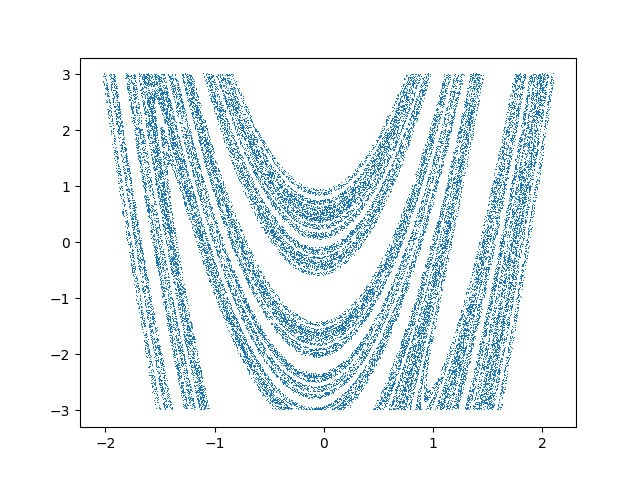
\includegraphics[width=6cm]{hsu/stable.png}}
		\subfigure[Variedade inst\'avel]{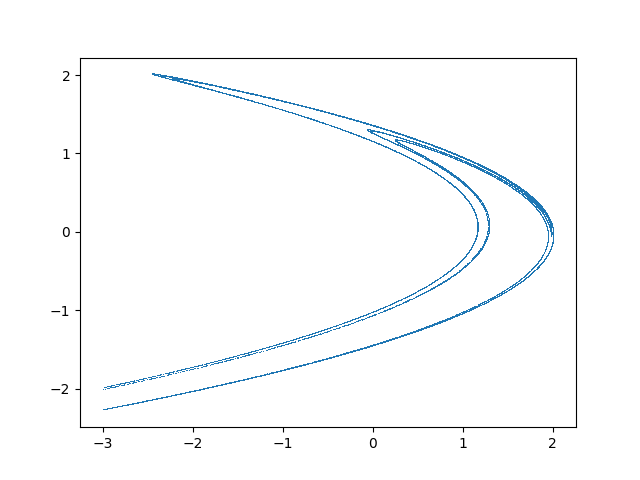
\includegraphics[width=6cm]{hsu/unstable.png}}
		\subfigure[Sela ca\'otica]{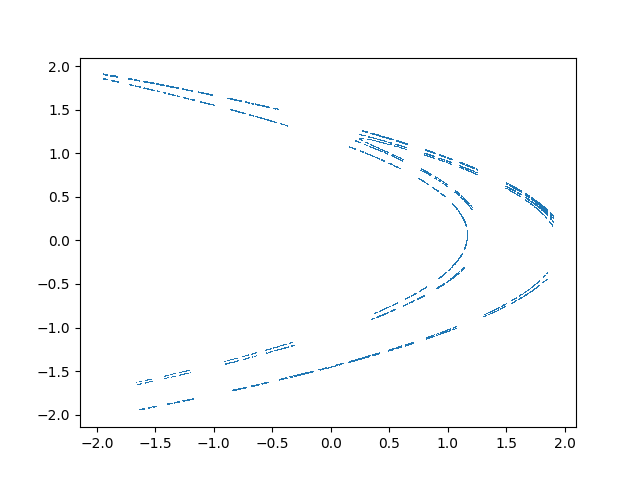
\includegraphics[width=6cm]{hsu/saddle.png}}
		\caption{Resultados do algoritmo de \textit{Sprinkler}}
		\label{fig:sprinkler_results}
	\end{figure}
	A figura da sela ca\'otica j\'a evidencia como ela de fato \'e um conjunto de Cantor.
	A figura \ref{fig:hsu_zoom} refor\c{c}a isso.
	\begin{figure}[H]
		\centering
		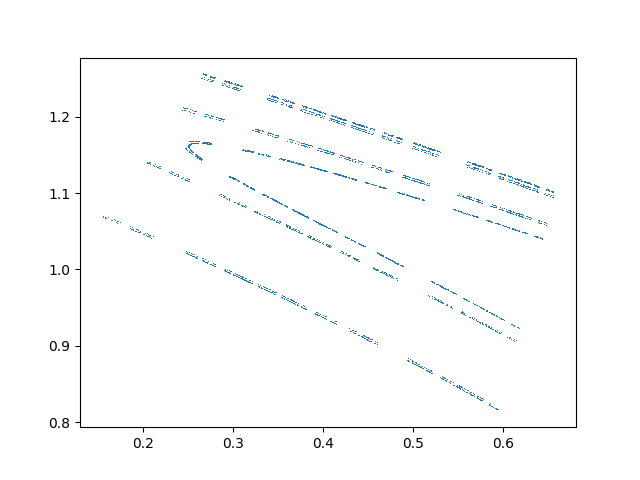
\includegraphics[width=8cm]{hsu/zoom.png}
		\caption{Zoom sobre uma parte da sela ca\'otica}
		\label{fig:hsu_zoom}
	\end{figure}
	E a \'ultima evid\^encia de que de fato o algoritmo funcionou est\'a na figura
	\ref{fig:hsu_inter}.
	\begin{figure}[H]
		\centering
		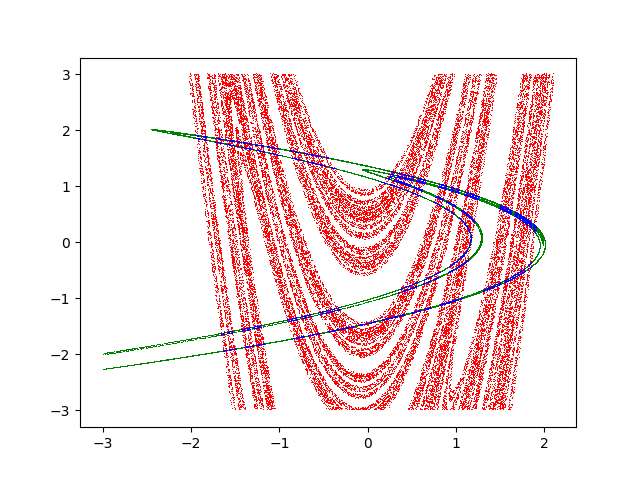
\includegraphics[width=8cm]{hsu/all.png}
		\caption{Impress\~ao dos tr\^es conjuntos numa mesma figura}
		\label{fig:hsu_inter}
	\end{figure}
	Nela, est\'a evidente como a sela ca\'otica encontrada de fato constitui interse\c{c}\~ao
	da variedade est\'avel com a inst\'avel.
	\section{Quest\~ao 2}
	Como se verificou no artigo, o mapa em quest\~ao \'e o seguinte, derivado
	do de \textit{Hen\'on}:
	\begin{equation}
		f(x, y) = (1.276 - x^2 + 0.3y, x)
		\nonumber
	\end{equation}
	Como existe em pauta, uma \'orbita de per\'iodo 7 que desempenha um papel importante,
	utilizou-se \textit{Python} para estimar numericamente os pontos fixos do mapa aplicado
	7 vezes, encontrando-se assim a \'orbita de per\'iodo 7. Para encontrar a variedade
	est\'avel que define as regi\~oes de restri\c{c}\~oes, primeiramente se determina
	a jacobiana do mapa de \textit{Hen\'on}:
	\begin{equation}
		D_f(x, y) = \left|\begin{array}{cc}
			-2x & 1\\
			0.3 & 0
		\end{array}\right|
		\nonumber
	\end{equation}
	Pode-se ent\~ao aplicar m\'etodos num\'ericos para encontrar a variedade est\'avel
	correspondente ao ponto da \'orbita peri\'odica, basta calcular o autovetor desta matriz.
	Todavia, o que foi feito at\'e agora somente foi capaz de encontrar a sela ca\'otica de fundo.
	A de banda n\~ao aparecia. Foi ent\~ao que se percebeu que a \'orbita peri\'odica de per\'iodo
	7 era sutilmente diferente da do artigo. Dessa forma, a divis\'oria da variedade est\'avel
	n\~ao era ideal para se gerar a sela ca\'otica de banda.

	Aparentemente haviam dois pontos fixos para o mapa de Hen\'on a s\'etima pot\^encia,
	e o do artigo era mais dif\'icil de se encontrar. Por\'em, percebeu-se que a sela ca\'otica
	de fundo que se tinha gerado estava congruente com a do artigo, e um dos pontos peri\'odicos
	estavam quase em cima da ponta desta sela ca\'otica. Portanto, utilizou-se essa ponta
	como chute inicial, e pode-se gerar a figura requisitada:
	\begin{figure}[H]
		\centering
		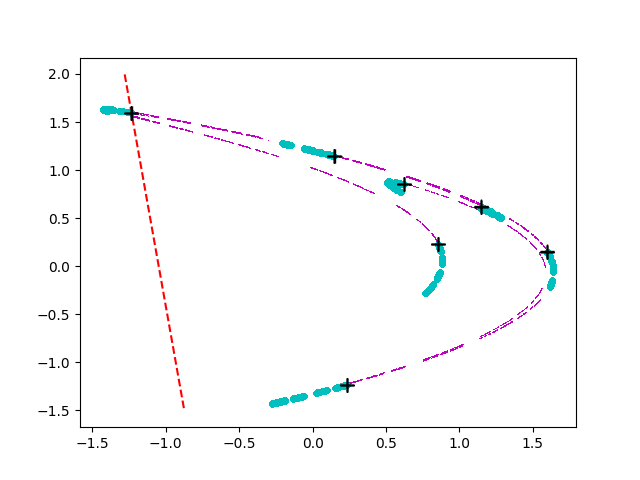
\includegraphics[width=8cm]{szabo/szabo.png}
		\caption{Fen\^omeno p\'os crise no mapa de \textit{Hen\'on}.}
	\end{figure}
	Percebe-se na figura as duas selas ca\'oticas bem descritas.
	\section{Quest\~ao 3}
	Gerou-se uma \'unica trajet\'oria, dividindo-a em ciclos de tamanho constante ao longo
	do tempo para se gerar uma s\'erie temporal para tr\^es valores diferentes de a: um
	antes da crise, um logo ap\'os, e um depois da crise. Gerou-se o valor de x no espa\c{c}o
	do mapa contra o ciclo atual, resultando nas seguintes figuras:
	\begin{figure}[H]
		\centering
		\subfigure[a = 1,266]{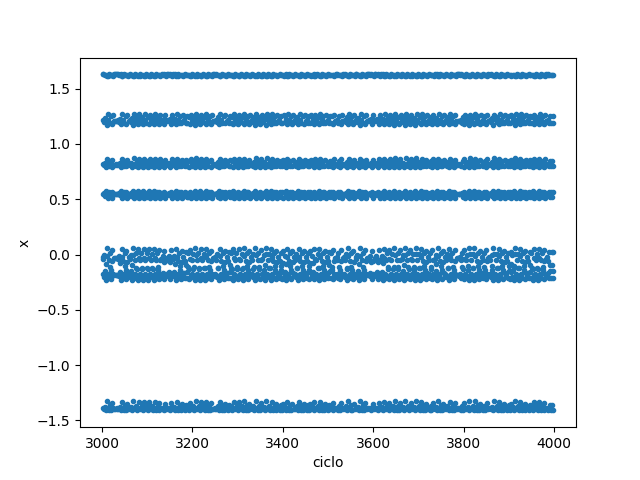
\includegraphics[width=4cm]{temporal_series/before_crisis.png}}
		\subfigure[a = 1,272]{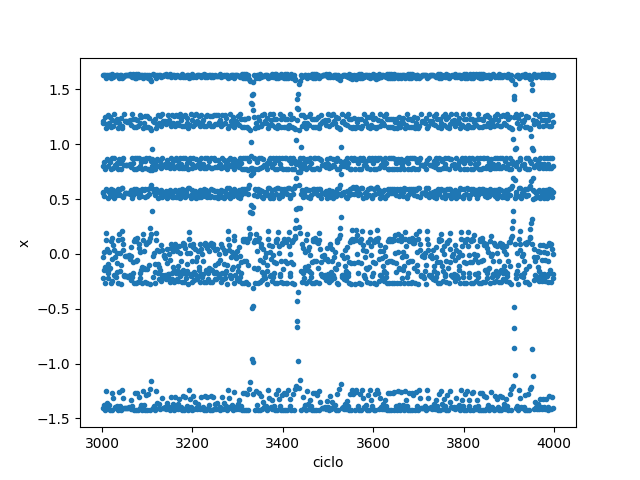
\includegraphics[width=4cm]{temporal_series/at_crisis.png}}
		\subfigure[a = 1,276]{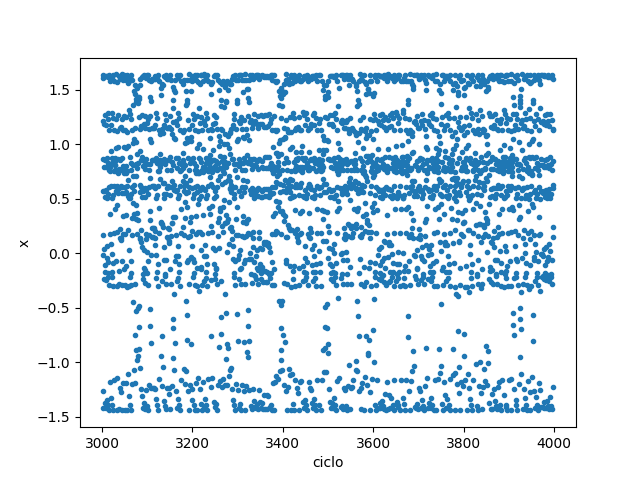
\includegraphics[width=4cm]{temporal_series/after_crisis.png}}
		\caption{Intermit\^encia caracter\'istica da crise interior no mapa de \textit{Hen\'on}.}
	\end{figure}
	Nelas, pode-se ver claramente como uma intermit\^encia induzida por crise interior aparece,
	junto com a crise, em virtude do acoplamento que ocorre entre as selas ca\'oticas, exatamente
	como \'e descrito na literatura.
\end{document}
